  \pagebreak
  \section{Actividad Práctica}
    Se propone medir la respuesta en frecuencia de un receptor FM mediante un generador de barrido y marcas, junto
    con un osciloscopio analógico. Los instrumentos de los cuales se hace uso son

    \begin{itemize}
      \item Generador de barrido y marcas LSW-250
      \item Osciloscopio analógico Hitachi V-665A
      \item Radio FM
    \end{itemize}
    
    El esquema de conexiones que se debe implementar con los dispositivos antes mencionados, se puede observar en
    la Figura~\ref{fig:EsquemaConexiones}.

    \begin{figure}[H]
      \centering
      \frame{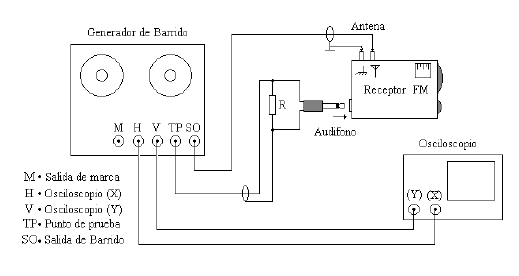
\includegraphics[width=0.6\textwidth]{Imagenes/ActividadPractica/EsquemaConexiones.png}}
      \caption{Esquema de conexiones para las mediciones.}
      \label{fig:EsquemaConexiones}
    \end{figure}
    
    
      \subsection{Calibración del dial del Generador de Barrido}
    A 

      \subsection{Características de detección}

      \subsection{Valores límtes de detección de sintonía}

